% \onecolumn






\clearpage
% \appendix


\begin{strip}
\begin{center}
\vspace{-5ex}
\textbf{\LARGE \bf
Adaptively Calibrated Critic Estimates for \\ Deep Reinforcement Learning} \\
\vspace{2ex}

% \Large{\bf- Supplementary Material -}\\
\Large{\bf- Appendix -}\\
\vspace{0.4cm}
\normalsize{Nicolai Dorka\hspace{1cm} Tim Welschehold \hspace{1cm} Joschka Bödecker\hspace{1cm} Wolfram Burgard}\\
\end{center}
\end{strip}

\setcounter{section}{0}
\renewcommand{\thesection}{A.\arabic{section}}
\makeatletter

\section{Proof of Theorem 1}

The estimator  $\qhatpi_{\beta^*}\sa$ was defined via
\begin{equation}
    \beta^* \sa = \argmin_{\beta \in [\bmin, \bmin]} \Bigg| \qhat_\beta \sa - \frac{1}{N} \sum_{i=1}^{N} R_i \sa  \Bigg| .
\end{equation}

To declutter the notation we drop the dependencies on the state-action pairs $\sa$ and the policy $\pi$.
Further we write $\Bar{R} = \frac{1}{N} \sum_{i=1}^{N} R_i $.
First note that the average of symmetrically distributed random variables is still a symmetric distributed random variable and hence 
$\Bar{R} $ is symmetrically distributed.
By assumption $\qhat_{\bmin}$ and $\qhat_{\bmax}$ have the same  distance to the true Q-value which is the mean $Q=\E[\Bar{R}] $, i.e. there is a distance real valued value $d$ such that
$Q = \qhat_{\bmin} +d = \qhat_{\bmax} -d$
Denote the tail probabilty  P($\Bar{R} < \qhat_{\bmin}) = p_t$.  Because of the symmetry and the same distance to the mean we also have that  $P(\Bar{R} > \qhat_{\bmax}) = p_t$.
In the computation of $\E [ \qhat_{\beta^*} ]$  we can differentiate three events.
If $\qhat_{\bmin} \leq \Bar{R} \leq \qhat_{\bmax}$ then $\qhat_{\beta^*} =\Bar{R}$, 
if $\qhat_{\bmin} \geq \Bar{R}$ then $\qhat_{\beta^*} =\qhat_{\bmin}$
and if $\qhat_{\bmin} \geq \Bar{R}$ then $\qhat_{\beta^*} =\qhat_{\bmax}$.
We denote the indicator function with $\idc{A}$, which is equal to $1$ if the event $A$ is true and $0$ otherwise.
Then we get

 
\begin{align*}
   \E \Big[ \qhat_{\beta^*} \Big] 
%   &= \E \Bigg[ \min_{\beta \in [\bmin, \bmin]} \Big| \qhat_\beta  - \Bar{R}   \Big| \Bigg] \\
%   &=  \E \Bigg[ \idc{\qhat_{\bmin} \leq \Bar{R} \leq \qhat_{\bmax}} 
%   \min_{\beta \in [\bmin, \bmin]} \Big| \qhat_\beta  - \Bar{R}  \Big| \Bigg]  \\
%   &~~~~+  \E \Bigg[ \idc{\qhat_{\bmin} \geq \Bar{R} }
%   \min_{\beta \in [\bmin, \bmin]} \Big| \qhat_\beta  - \Bar{R}  \Big| \Bigg] \\
%   &~~~~+ \E \Bigg[ \idc{\qhat_{\bmax} \leq \Bar{R} }
%   \min_{\beta \in [\bmin, \bmin]} \Big| \qhat_\beta  - \Bar{R}  \Big| \Bigg] \\
   &= \E \Bigg[ \idc{\qhat_{\bmin} \leq \Bar{R} \leq \qhat_{\bmax}} \Bar{R}  \Bigg]  \\
  &~~~~+  \E \Bigg[ \idc{\qhat_{\bmin} \geq \Bar{R} }  \qhat_{\bmin} \Bigg] \\
  &~~~~+  \E \Bigg[ \idc{\qhat_{\bmax} \leq \Bar{R} }  \qhat_{\bmax}  \Big| \Bigg]  \\
%   +  \E \Bigg[ \idc{\qhat_{\bmin} \geq \Bar{R} }  \qhat_{\bmin} \Bigg] 
%   +  \E \Bigg[ \idc{\qhat_{\bmax} \leq \Bar{R} }  \qhat_{\bmax}  \Big| \Bigg]  \\
   &= (1-2p_t) \cdot \E[\Bar{R}] + p_t \E\Big[\qhat_{\bmin}\Big] + p_t \E\Big[\qhat_{\bmax}\Big] \\
   &= (1-2p_t) Q + p_t \qhat_{\bmin}+ p_t \qhat_{\bmax}\\
   &= (1-2p_t) Q + p_t (Q-d) + p_t (Q+d)\\
   &= (1-2p_t) Q + 2p_t Q + p_t(d-d) \\
   &= Q.
\end{align*}




\section{Pseudocode}
\label{app:pseudocode}


The pseudocode for ACC applied to TQC is in Algorithm \ref{alg:acc_applied_to_tqc}.
As the number of dropped targets per network is given by $d= d_{\max} - \beta $, we state the pseudocode in terms of the parameter $d$ instead of $\beta$. 


\begin{algorithm}[t]
   \caption{ACC - Applied to TQC}
   \label{alg:acc_applied_to_tqc}
\begin{algorithmic}
   \STATE {\bfseries Initialize:} $d$ the bias controlling parameter, $\alpha$ the learning rate for $d$, $T_d$ the minimum number of steps between updates to $d$, $T_d^{init}$  the initial steps before $d$ is updated,
   $S_R$ the size from which on episodes are removed from the batch storing the most recent returns, moving average parameter $\tau_d$, $t_d = 0$
   \FOR{$t=1$ {\bfseries to} total number of environment steps}
   \STATE Interact with environment according to $\pi$, store transitions in replay buffer $\mathcal{B}$ and, increment $t_d \pluseq 1$
    \IF{episode ended}
   \STATE Store observed returns $R\sa$ and corresponding state-action pairs $\sa$ in $\mathcal{B}_R$

   
   \IF{ $t_d >= T_d$ \textbf{and} $t > T_d^{init}$}
   \STATE $C = \sum_{ (s,a, R) \in \mathcal{B}_R} \Big[   Q \sa - R \sa  \Big]$,     $ma = (1-\tau_d) ma + \tau_d C$
   \STATE $d = d + \alpha \frac{C}{ma}$, clip $d$ in interval $[0, d_{max}]$, set $t_d=0$
    \STATE Remove the oldest episodes from $\mathcal{B}_R$ until there are at most $S_R$ left
   \ENDIF
   \ENDIF
%   \FOR{$j=1$ {\bfseries to} number Q-updates per environment step}
   \STATE Sample mini-batch from $\mathcal{B}$
   \STATE Update critic $Q$ as in TQC, where $dN$ (rounded to the next integer) number of targets are dropped from the set of pooled targets 
   \STATE Update policy $\pi$ as in TQC 
%   \ENDFOR
  \ENDFOR
\end{algorithmic}
\end{algorithm}


 


\section{Using Fewer Critic Networks for Faster Runtime}
\label{app:2_nets}

\begin{figure*}[t]
\centering
  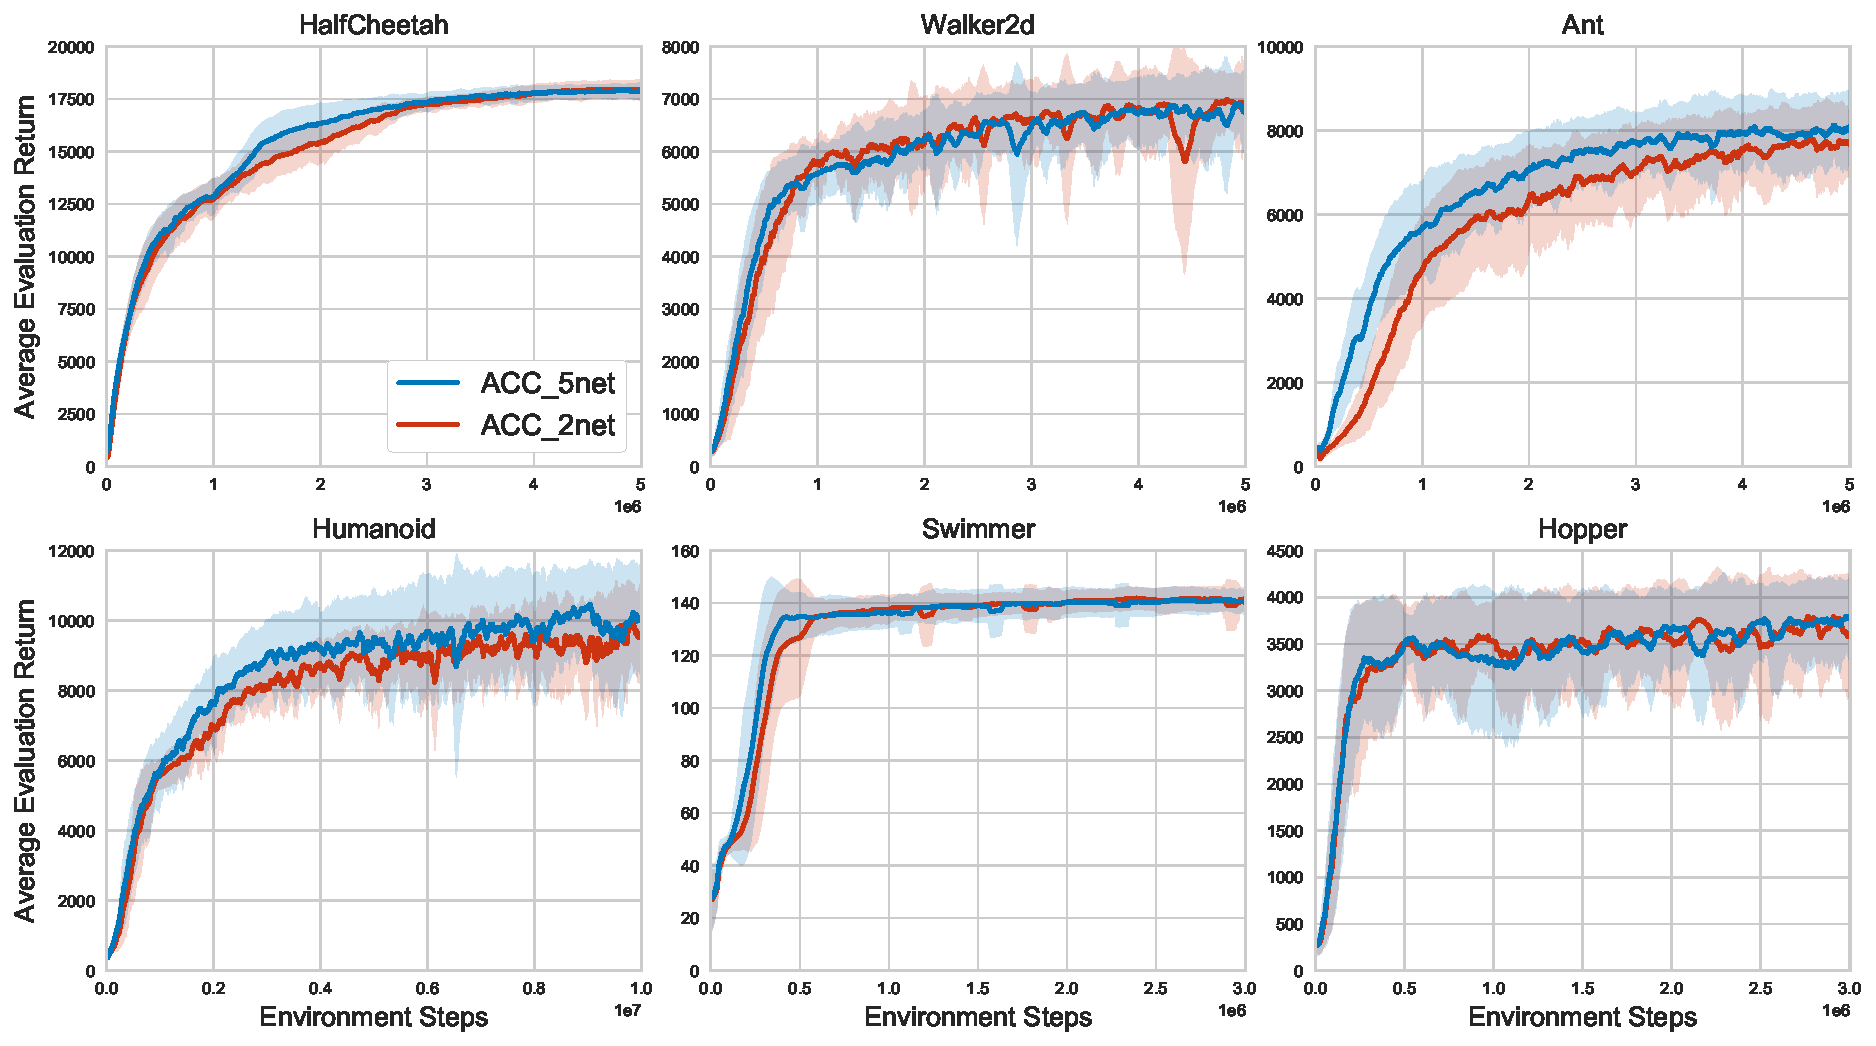
\includegraphics[width=.8\linewidth]{images/ablation/2net_one_fig.pdf}
\caption{The mean $\pm$ standard deviation over $10$ trials. 
Results with different choices for the number of critic networks for each algorithm. }
\label{fig:num_critic_nets}
\end{figure*}
Using $5$ critic networks - the default in TQC - to approximate the value function leads to a high runtime of the algorithm. It is possible to trade off performance against runtime by changing the number of critic networks. We evaluated ACC applied to TQC with $2$ networks and compare it to the standard setting with $5$ networks in Figure \ref{fig:num_critic_nets}. The results show that reducing the number of critic networks to $2$ leads only to a small drop in performance while the runtime is more than $2$ times faster.







\section{Hyperparameters}
\label{app:hyperparameter}

At the beginning of the training we initialize $\beta = 2.5$ and set the step size parameter to $\alpha=0.1$.
After $T_\beta = 1000$ steps since the last update and when the next episode finishes, $\beta$ is updated with a batch that stores the most recent state-action pairs encountered in the environment and their corresponding observed discounted returns. 
The choice of $T_\beta$ was motivated by the fact that the maximum duration of an episode is $1000$ steps for the considered environments.
After every update of $\beta$ the oldest episodes in this stored batch are removed until there are no more than $5000$ state-action pairs left. This means that on average $\beta$ is updated with a batch whose size is a bit over $5000$. 
The updates of $\beta$ are started as soon as $25000$ environment steps as completed and
the moving average parameter in the normalization of the $\beta-$update is set to $0.05$. 
The  first $5000$ environment interactions are generated with a random policy after which learning starts.
Apart from that all hyperparameters are the same as in TQC with $N=5$ critic networks.
In Table \ref{tab:hyperparameter} we list all hyperparameters of ACC applied to TQC.

In the following we also desribe the process of hyperparameter selection.
The range of values $d$ is allowed to take is set to the interval $[0,5]$ as it includes the optimal hyperparameters for TQC from all environments, which are in the set $\{0,2,5\}$. We did not try higher values than $5$.
The initial value for number of dropped targets per network was set to $2.5$ as this value is in the middle of the allowed range and did not evaluated other choices.
The learning rate $\alpha$ of $d$ was set to $0.1$ based on visual inspection of how fast $d$ changes. We  evaluated $\alpha=0.05$ for a small subset of tasks and seeds, but $\alpha=0.1$ gave slightly better results.
$T_d$ was set to $1000$ as the episode length is $1000$ and we did not evaluate other choices.
For $T_d^{init}$ we evaluated the choices $10000$ and $25000$ on a small subset of environments and seeds and did not found a big impact on performance. As $d$ changes very quickly in the beginning we chose $T_d^{init}=25000$.
For $S_R$ we evaluated the choices $1000$ and $5000$ also on a small subset of environments and seeds and found $5000$ to perform slightly better.
We did not tune the moving average parameter and set it to $\tau_d = 0.05$.
For all hyperparameters for which we evaluated more than one choice we do not have definite results as the number of seeds and environments were limited.
The hyperparameters shared with TQC were not changed.
For TD3 and SAC we used the hyperparameters from the respective papers.




\begin{table*}[t]
\caption{Hyperparameters values.}
\label{tab:hyperparameter}
\vskip 0.15in
\begin{center}
\begin{small}
\begin{sc}
\begin{tabular}{lccc}
\toprule
Hyperparameter & \multicolumn{3}{c}{ACC} \\
\midrule
Optimizer & \multicolumn{3}{c}{Adam} \\
Learning rate & \multicolumn{3}{c}{\num{3e-4}} \\
Discount $\gamma$ & \multicolumn{3}{c}{0.99} \\
Replay buffer size & \multicolumn{3}{c}{\num{1e6}} \\
Number of critics $N$ & \multicolumn{3}{c}{5} \\
Number of atoms $M$ & \multicolumn{3}{c}{25}\\
Huber loss parameter  & \multicolumn{3}{c}{1} \\
Number of hidden layers in critic networks & \multicolumn{3}{c}{3}\\
Size of hidden layers in critic networks & \multicolumn{3}{c}{512} \\
Number of hidden layers in policy network & \multicolumn{3}{c}{2} \\
Size of hidden layers in policy network & \multicolumn{3}{c}{256} \\
Minibatch size & \multicolumn{3}{c}{256} \\
Entropy target  &  \multicolumn{3}{c}{$- \dim \mathcal{A}$} \\
Nonlinearity & \multicolumn{3}{c}{ReLU} \\
Target smoothing coefficient  & \multicolumn{3}{c}{0.005} \\
Target updates per critic gradient step & \multicolumn{3}{c}{1} \\
Critic gradient steps per iteration & \multicolumn{3}{c}{1} \\
Actor gradient steps per iteration & \multicolumn{3}{c}{1} \\
Environment steps per iteration & \multicolumn{3}{c}{1} \\
\midrule
Initial value for number of dropped targets per network & \multicolumn{3}{c}{2.5} \\
Maximum value for $d$ denoted $d_{\max}$ & \multicolumn{3}{c}{5} \\
Minimum value for $d$ denoted $d_{\min}$ & \multicolumn{3}{c}{0} \\
Learning rate for $d$ denoted $\alpha$ & \multicolumn{3}{c}{0.1} \\
Minimum number of steps between updates to $d$ denoted $T_d$ & \multicolumn{3}{c}{1000} \\
Initial number of steps before $d$ is updated denoted $T_d^{init}$ & \multicolumn{3}{c}{25000} \\
Limiting size for batch used to update $d$ denoted $S_R$ & \multicolumn{3}{c}{5000} \\
Moving average parameter $\tau_d$ & \multicolumn{3}{c}{0.05} \\
\midrule
\midrule
Hyperparameter in Sample Efficient Experiment & ACC\_1q & ACC\_2q & ACC\_4q \\
\midrule
Critic gradient steps per iteration & 1 & 2 & 4 \\
Actor gradient steps per iteration & 1 & 1 & 1 \\
Target updates per critic gradient step & 1 & 1 & 1\\
\bottomrule
\end{tabular}
\end{sc}
\end{small}
\end{center}
\vskip -0.1in
\end{table*}






\section{Potential Limitations}
One limitation of our work is that ACC can not be applied in the offline RL setting, as ACC also uses on-policy data.
Furthermore, in the stated form ACC relies on the episodic RL setting. However, we believe that ACC could potentially be adapted to that setting. 
It is also not entirely clear how the algorithm would perform in the terminal reward setting, where a reward of for example $1$ is given upon successful completion of a specific task. While we do not have experiments for such environments we imagine that the positive effect of ACC could diminish as the true Q-values of states closer to the start of the episode are almost zero because of the discounting. 




\section{Analysis of the ACC Parameter}
\label{app:analysis_acc_parameter}

\begin{figure*}[b]
  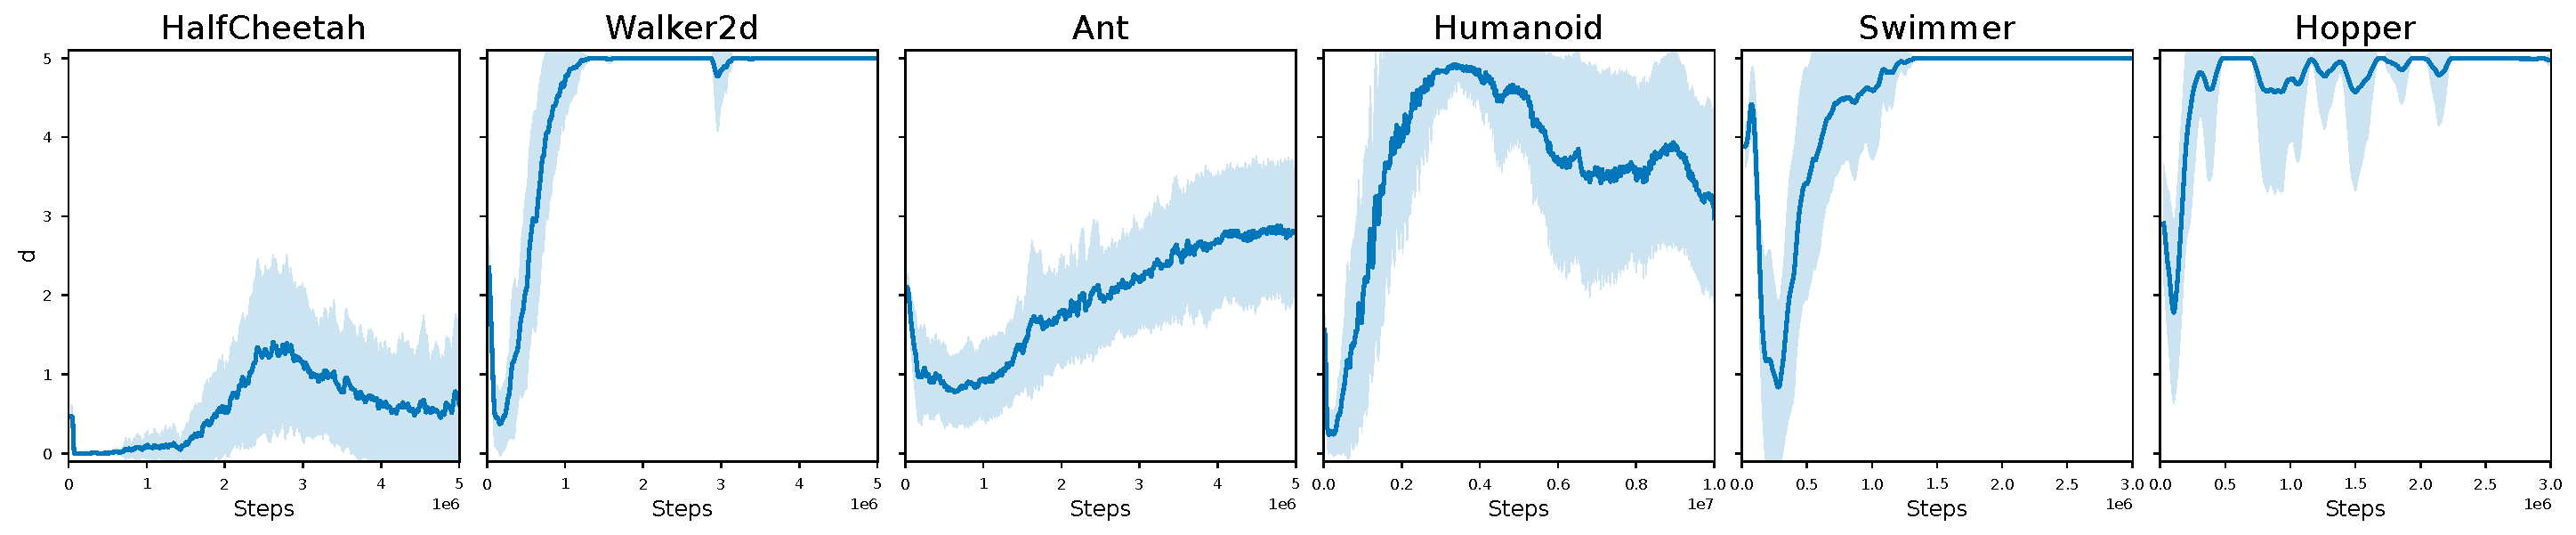
\includegraphics[width=1\linewidth]{images/analysis/visualize_beta_all_envs.pdf}
  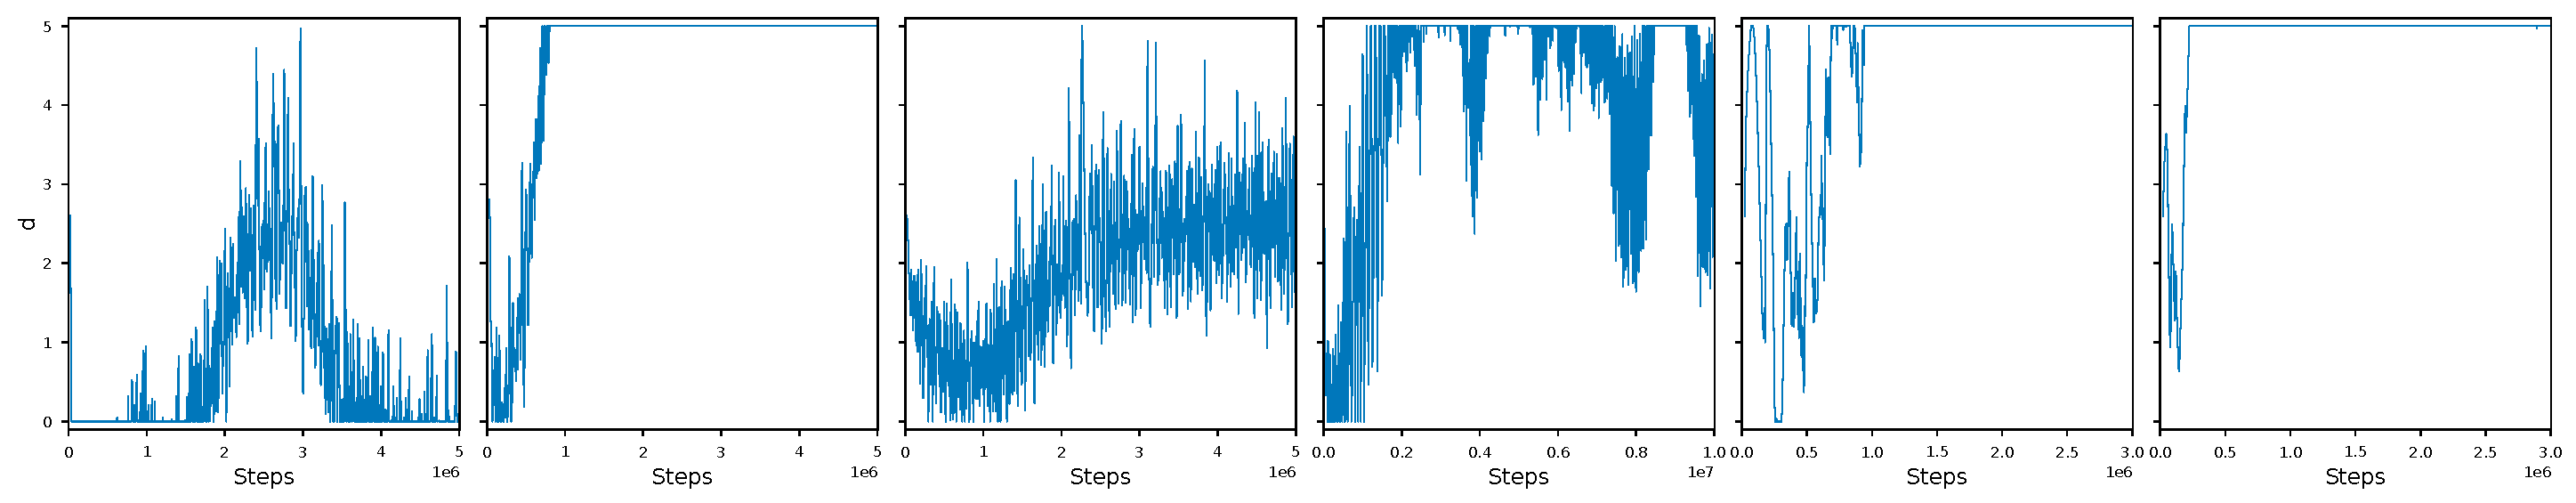
\includegraphics[width=1\linewidth]{images/analysis/visualize_beta_one_run_all_envs.pdf}
\caption{Development of the number of dropped targets per network $d=d_{max}-\beta$ in ACC over time for different environments. The top row shows the mean (thick line) and standard deviation (shaded area) over the $10$ trials where for readability a uniform filter of size $15$ is used.
The bottom row shows the unfiltered development for one of the seeds.}
\label{fig:num_dropped_targets_all_envs}
\end{figure*}




To better understand the hidden training dynamics of ACC we show in 
Figure \ref{fig:num_dropped_targets_all_envs}
how the number of dropped targets per network $d=d_{max}-\beta$ evolves during training. 
To do so we plotted $d$ after every $5000$ steps during the training of ACC.
From the top row the first observation is that per environment the results are similar over the $10$ seeds as can be seen from the relatively low standard deviation. We show the single runs for all seeds in the appendix to further support this observation.
However, there are large differences between the environments which supports the argument that it might not be possible to find a single hyperparameter that works well on a wide variety of different environments.
Another point that becomes clear from the plots is that the optimal amount of overestimation correction might change over time during the training even on a single environment.

In the bottom row of Figure \ref{fig:num_dropped_targets_all_envs} we plotted the evolution of $d$ for one of the $10$ trials in order to shed light on the actual training mechanics of a single run without lost information due to averaging.
For each environment there is a trend but $d$ is also fluctuating to a certain degree.
While this shows that the initial value of $d$ is not very important as the value quickly changes, this also highlights another interesting aspect of ACC. 
The rollouts give highly fluctuating returns. The parameter $d=d_{max}-\beta$ is changing more slowly and picks up the trend. So a lot of the variance of the returns is filtered out in ACC by incorporating on-policy samples via the detour over $\beta$.
This leads to relatively stable TD targets computed from $\qbeta$ while an upbuilding under- or overestimation is prevented as $\beta$ picks up the trend. On the other hand, if $\beta$ would change too slowly the upbuilding of the bias might not be stopped.





